\documentclass[tikz, border=10pt]{standalone}
%%%<
\usepackage{verbatim}
%%%>
\usetikzlibrary{arrows}
\begin{document}
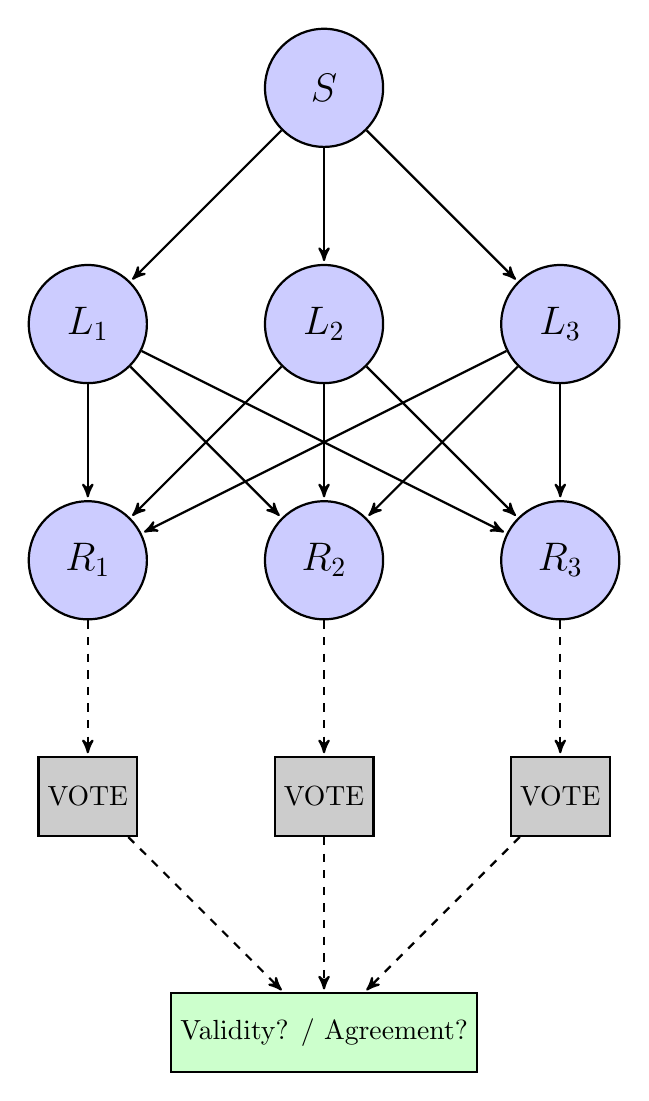
\begin{tikzpicture}[->,>=stealth',shorten >=1pt,auto,node distance=3cm,
  thick,main node/.style={circle,fill=blue!20,draw,
  font=\sffamily\Large\bfseries,minimum size=15mm},
  vote node/.style={rectangle,draw,fill=black!20,minimum size=10mm},
  prop node/.style={rectangle,draw,fill=green!20,minimum size=10mm}]

  \node[main node] (S)                {$S$};
  \node[main node] (L2) [below of=S]  {$L_2$};
  \node[main node] (L1) [left of=L2]  {$L_1$};
  \node[main node] (L3) [right of=L2] {$L_3$};
  \node[main node] (R2) [below of=L2] {$R_2$};
  \node[main node] (R1) [left of=R2]  {$R_1$};
  \node[main node] (R3) [right of=R2] {$R_3$};

  \node[vote node] (V1) [below of=R1] {VOTE};
  \node[vote node] (V2) [below of=R2] {VOTE};
  \node[vote node] (V3) [below of=R3] {VOTE};

  \node[prop node] (P)  [below of=V2] {Validity? / Agreement?};

  \path[every node/.style={font=\sffamily\small,
        fill=white,inner sep=1pt}]
    % source broadcast
    (S) edge (L1)
    (S) edge (L2)
    (S) edge (L3)
    % relay 1 broadcast
    (L1) edge (R1)
    (L1) edge (R2)
    (L1) edge (R3)
    % relay 2 broadcast
    (L2) edge (R1)
    (L2) edge (R2)
    (L2) edge (R3)
    % relay 3 broadcast
    (L3) edge (R1)
    (L3) edge (R2)
    (L3) edge (R3);

    %\path[->, >=stealth', shorten >=1pt, auto, thick, dashed]
    \draw[->, thick, dashed] (R1) to (V1);
    \draw[->, thick, dashed] (R2) to (V2);
    \draw[->, thick, dashed] (R3) to (V3);

    \draw[->, thick, dashed] (V1) to (P);
    \draw[->, thick, dashed] (V2) to (P);
    \draw[->, thick, dashed] (V3) to (P);

\end{tikzpicture}
\end{document}
